\documentclass[10pt,a4paper]{article}
\usepackage[utf8]{inputenc}
\usepackage{amsmath}
\usepackage{amsfonts}
\usepackage{amssymb}
\usepackage{amsthm}
\usepackage{float}
\usepackage{mathtools}
\usepackage{geometry}[margin=1in]
\usepackage{xspace}
\usepackage{tikz}
\usepackage{mathrsfs}
\usetikzlibrary{shapes, arrows, decorations.pathmorphing}
\usepackage[parfill]{parskip}
\usepackage{subcaption}
\usepackage{stmaryrd}
\usepackage{marvosym}
\usepackage{dsfont}

\newcommand{\st}{\text{ s.t. }}
\newcommand{\contr}{\lightning}
\newcommand{\im}{\mathfrak{i}}
\newcommand{\R}{\mathbb{R}}
\newcommand{\Q}{\mathbb{Q}}
\newcommand{\C}{\mathbb{C}}
\newcommand{\F}{\mathbb{F}}
\newcommand{\K}{\mathbb{K}}
\newcommand{\N}{\mathbb{N}}
\newcommand{\Z}{\mathbb{Z}}
\renewcommand{\H}{\mathds{H}}
\newcommand{\nequiv}{\not\equiv}
\newcommand{\powset}{\mathcal{P}}
\renewcommand{\th}[1][th]{\textsuperscript{#1}\xspace}
\newcommand{\from}{\leftarrow}
\newcommand{\legendre}[2]{\left(\frac{#1}{#2}\right)}
\newcommand{\ow}{\text{otherwise}}
\newcommand{\imp}[2]{\underline{\textit{#1.}$\implies$\textit{#2.}}}
\let\oldexists\exists
\renewcommand{\exists}{\oldexists\;}
\renewcommand{\hat}{\widehat}
\renewcommand{\tilde}{\widetilde}
\newcommand{\one}{\mathds{1}}
\newcommand{\under}{\backslash}
\newcommand{\injection}{\hookrightarrow}
\newcommand{\surjection}{\twoheadrightarrow}
\newcommand{\jacobi}{\legendre}
\newcommand{\floor}[1]{\lfloor #1 \rfloor}
\newcommand{\ceil}[1]{\lceil #1 \rceil}
\newcommand{\cbrt}[1]{\sqrt[3]{#1}}

\DeclareMathOperator{\ex}{ex}
\DeclareMathOperator{\id}{id}
\DeclareMathOperator{\upper}{Upper}
\DeclareMathOperator{\dom}{dom}

\DeclareMathOperator{\charr}{char}
\DeclareMathOperator{\Image}{im}
\DeclareMathOperator{\ord}{ord}
\DeclareMathOperator{\lcm}{lcm}
\let\emph\relax
\DeclareTextFontCommand{\emph}{\bfseries\em}

\newtheorem{theorem}{Theorem}[section]
\newtheorem{lemma}[theorem]{Lemma}
\newtheorem{corollary}[theorem]{Corollary}
\newtheorem{proposition}[theorem]{Proposition}
\newtheorem{conjecture}[theorem]{Conjecture}

\tikzset{sketch/.style={decorate,
 decoration={random steps, amplitude=1pt, segment length=5pt}, 
 line join=round, draw=black!80, very thick, fill=#1
}}

\title{Algebraic Geometry}
\begin{document}
\maketitle

\setcounter{section}{-1}

\section{Introduction}
What is algebraic geometry? Broadly speaking, it is the study of the geometry of solutions to systems of polynomial equations. For example, in $\R^2$, if we have the set $X$ of solutions to $\{(x,y)\in \R^2 : x^2+y^2 = 1\}$, then we know that this set forms a circle, and we know lots of geometric facts about circles. If we take a more complicated function, such as $y^2 = x^3-x$, we get something that looks like:
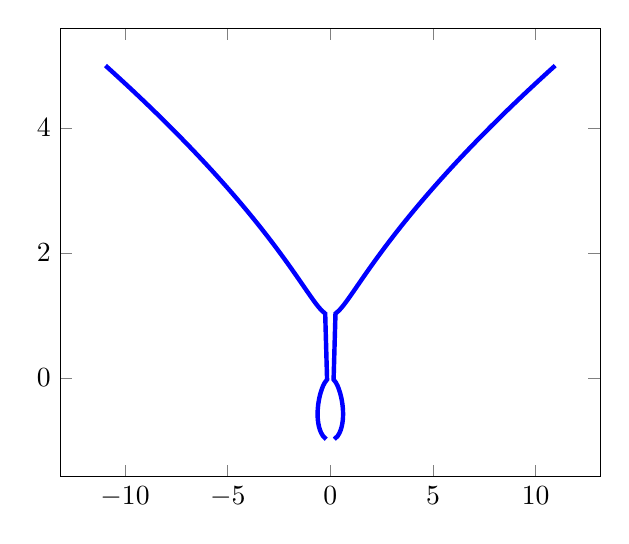
\begin{tikzpicture}% fill this in
\begin{axis}
\addplot[blue, ultra thick, samples=200] ({(x^3-x)^(0.5)}, x);
\addplot[blue, ultra thick, samples=200] ({-(x^3-x)^(0.5)}, x);
\end{axis}
\end{tikzpicture}

If we instead think about complex solutions, we get something of the form of a torus minus a single point, with another rich geometric structure.

In $\C^3$, if $X = \{(x,y,z) \in \C^3 : x^3 + y^3 + z^3 = 1\}$, then $X$ contains 27 lines: $x = -\xi^m y, z = \xi^n$ for $i,j \in \{0,1,2\}$ gives 9 of them, and the other 18 come by rotating $x,y,z$ in this linear system.

In $\R^3$, consider the equation $1+x^3+y^3+z^3 = (1+x+y+z)^3$. %find pic of this

\section{Basic Setup}
Fix a field $K$. We define an \emph{affine n-space over K} to be $\mathbb{A}^n \coloneqq K^n$. Let $A \coloneqq K[x_1,x_2,\ldots,x_n]$ be the polynomial ring in $n$ variables over $K$, and let $S \subseteq A$ be a subset of $A$. We then define $Z(S)$, the \emph{zero set of S} to be the set of all $n$-tuples $(a_1,\ldots,a_n) \in \mathbb{A}^n$ where $f(a_1,\ldots,a_n) = 0$ for all $f \in S$.

\begin{proposition}
\item
\begin{enumerate}
\item $Z(\{0\}) = \mathbb{A}^n$
\item $Z(A) = \emptyset$
\item $Z(S_1\cdot S_2) = Z(S_1) \cup Z(S_2)$, where $S_1\cdot S_2 = \{f_1\cdot f_2 : f_1 \in S_1, f_2 \in S_2\}$.
\item Let $I$ be an index set, $S_i \subseteq A$ for each $i \in I$. Then $\bigcap_{i \in I} Z(S_i) = Z(\bigcup_{i \in I} S_i)$
\end{enumerate}
\end{proposition}
\begin{proof} \textit{1., 2.} are obvious
\begin{enumerate}
\item If $p \in Z(S_1) \cup Z(S_2)$, then either $p \in Z(S_1)$ or $p \in Z(S_2)$. If $p \in Z(S_1)$, then $f_1(p) = 0$ for all $f_1 \in S_1$, and so $f_1(p)\cdot f_2(p) = 0$ for all $f_1 \in S_1, f_2 \in S_2$, so $p \in Z(S_1\cdot S_2)$, and similarly for if $p \in Z(S_2)$.

Conversely, suppose that $p \in Z(S_1\cdot S_2)$, and $p \notin Z(S_1)$. Then there is some $f_1 \in S_1$ with $f_1(p) \neq 0$. But $f_1(p)\cdot f_2(p) = 0$ for all $f_2 \in S_2$, and so $f_2(p) = 0$ for all $f_2 \in S_2)$, so $p \in Z(S_2)$.

\item If $p \in Z(S_i)$ for all $i \in I$, then $f_i(p) = 0$ for all $f_i \in S_i$, and so for all $f \in \bigcup_{i} S_i$, so $p \in Z(\bigcup_{i \in I}S_i)$.

Conversely, if $p \in Z(\bigcup_i S_i)$, then $f(p) = 0$ for all the polynomials in $\bigcup_i S_i$, and so $p \in \bigcap_i S_i$.
\end{enumerate}
\end{proof}
These four properties should remind you of the four axioms for a topology.

A subset of $\mathbb{A}^n$ is \emph{algebraic} if it of the form $Z(S)$ for some $S\subseteq A$. A \emph{Zariski open set} in $\mathbb{A}^n$ is a set of the form $\mathbb{A}^n \setminus Z(S)$ for some $S \subseteq \mathbb{A}^n$. This proposition tells us that the Zariski open sets define a topology on $\mathbb{A}^n$, called the \emph{Zariski topology}.

\underline{Examples:}
\begin{enumerate}
\item $K = \C$. The Zariski open (or closed) subsets of $\C^n = \mathbb{A}^n$ are in particular open (or closed) in the usual Euclidean sense, but not vice versa.
\item For any $K$, consider $\mathbb{A}^1, A = K[x], S \subseteq K[x]$. If $S$ has a non-zero element, then $Z(S)$ is finite. Thus the closed sets are the finite subsets of $\mathbb{A}^1$, and all of $\mathbb{A}^1$. The open sets are $\emptyset$ and all the co-finite sets (i.e. sets with finite complement).
\end{enumerate}

Recall that, if $A$ is any commutative ring with $S \subseteq A$ a subset, then the \emph{ideal generated by S} is the ideal $A \supseteq \angle{S} = \{\sum_{i=1}^q f_ig_i : q \geq 0, f_i \in S, g_i \in A\}$, or the smallest ideal of $A$ containing $S$.

\begin{lemma}
Let $S \subseteq A = K[x_1, \ldots, x_n]$. Then $Z(S) = Z(\angle{S})$.
\end{lemma}
\begin{proof}
If $p \in Z(S)$, then for $f_1, \ldots, f_q \in S; g_1, \ldots, g_q \in A$ we have:
\begin{align*}
\left(\sum_{i=1}^q f_ig_i\right)(p) = \sum_{i=1}^q f_i(p)g_i(p) = \sum_{i=1}^p 0\cdot g_i(p) = 0
\end{align*}
So $p \in Z(\angle{S})$, and so $Z(S)\subseteq Z(\angle{S})$. 

\hspace*{-1em}The other inclusion follows from the fact that $S \subseteq \angle{S}$, we must have $Z(\angle{S}) \subseteq Z(S)$.
\end{proof}

Let $X \subseteq \mathbb{A}^n$ be a subset. Define $I(X) \coloneqq \{f \in A : f(p) = 0 \;\forall p \in X\}$, the \emph{ideal of X}. Note that $I(X)$ is indeed an ideal, since if $f, g \in I(X)$ then $f+g \in I(X)$, and if $f \in I(X), g \in A$, then $f\cdot g \in I(X)$. Note that if $S_1\subseteq S_2 \subseteq A_1$, then $Z(S_2) \subseteq Z(S_1)$, and if $X_1 \subseteq X_2$, then $I(X_2) \subseteq I(X_1)$.

The \emph{radical} of an ideal $I \subset A$ is the set $\sqrt{I} \coloneqq \{x \in A: \exists n\in\N \st x^n \in I\}$. This is defined in general for any commutative ring $A$, not just polynomial rings.

\begin{lemma}
$\sqrt{I}$ is an ideal.
\end{lemma}
\begin{proof}
If $f, g \in \sqrt{I}$, there is $n, m$ such that $f^n, g^m \in I$. Then $(f+g)^{m+n} = \sum_{i=0}^{m+n} \binom{m+n}{i}f^i g^{m+n-i}$. Now for each term in this sum, either we have $i \geq n$ or $m+m-i\geq m$, and so one of these terms is in $I$. Hence by the closure rules for ideals, $(f+g)^{m+n} \in I$, so $f+g \in \sqrt{I}$. Given $f \in \sqrt{I}, g \in A$, we have $(fg)^n = f^n g^n$, and $f^n \in I \implies f^ng^n \in I$, so $fg \in \sqrt{I}$.
\end{proof}

\begin{proposition}
\item
\begin{enumerate}
\item If $X \subseteq \mathbb{A}^n$ is algebraic, then $Z(I(X)) = X$.
\item If $I \subseteq A$ is an ideal, then $I(Z(I)) \supseteq \sqrt{I}$.
\end{enumerate}
\end{proposition}
\begin{proof}
\item
\begin{enumerate}
\item Since $X$ is algebraic $X = Z(I)$ for some $I \subseteq A$. Certainly $I \subseteq I(X)$, and so $Z(I(X)) \subseteq Z(I) = X$. But $X \subseteq Z(I(X))$ trivially, and so $X = Z(I(X))$.

\item If $f \in \sqrt{I}$, then $f^n \in I$ for some $n$, and so $f^n$ vanishes on $Z(I)$, thus $f$ vanishes on $Z(I)$. Hence $f \in I(Z(I))$.
\end{enumerate}
\end{proof}
\begin{theorem}[Hilbert Nullstellensatz]
Let $K$ be algebraically closed. Then $I(Z(I)) = \sqrt{I}$.
\end{theorem}
\begin{proof}
Deferred until later.
\end{proof}

\hspace*{-1em}\underline{Example:} If $K = \R$, $I = \angle{x^2+y^2+1} \subseteq \R[x,y]$, then $Z(I) = \emptyset$, so $I(Z(I)) = \R[x,y] \neq \sqrt{I}$.

\hspace*{-1em}We define an \emph{affine (algebraic) variety} to be an algebraic subset of $\mathbb{A}^n$. Very often we can decompose affine varieties into smaller subsets. For instance, $Z(\angle{xy}) = + = - \cup | = Z(\angle{x}) \cup Z(\angle{y})$. If $Y \subseteq X$ is a non-empty closed subset, then we say $Y$ is \emph{irreducible} if whenever $Y = Y_1 \cup Y_2$ with $Y_1, Y_2$ closed, then either $Y_1 = Y$ or $Y_2 = Y$.  In the Euclidean topology on $\C^n$, the irreducible subsets are single points, but under the Zariski topology they are much more interesting. We will now turn to the question of identifying when an algebraic set is irreducible.

\begin{proposition}
If $X_1, X_2 \subseteq \mathbb{A}^n$, then $I(X_1 \cup X_2) = I(X_1) \cap I(X_2)$.
\end{proposition}
\begin{proof}
Since $X_1, X_2 \subseteq X_1 \cup X_2, I(X_1 \cup X_2) \subseteq I(X_1), I(X_2)$. Hence $I(X_1 \cup X_2) \subseteq I(X_1) \cap I(X_2)$.

Conversely, if $f \in I(X_1) \cap I(X_2)$, then $f$ vanishes on both $X_1$ and $X_2$, and so on all of the union. So $I(X_1) \cap I(X_2) \subseteq I(X_1 \cup X_2)$.
\end{proof}

Recall that an ideal $P \subseteq A$ of a commutative ring is said to be \emph{prime} if it is not the whole ring, and whenever $fg \in P$, either $f \in P$ or $g \in P$.

\begin{lemma}
Let $P \subseteq A$ be prime, and $I_1, \ldots, I_n \subseteq A$ be ideals. Suppose that $P \supseteq \bigcap_i I_i$. Then there is some $i$ such that $P \supseteq I_i$, and if equality holds in either then it holds in both.
\end{lemma}
\begin{proof}
Suppose $P \nsupseteq I_i$ for any $i$, so for all $i$ there is some $x_i \in I_i \setminus P$. Then $x = \prod_i x_i \in I_i$ for all $i$, so $x \in \bigcap_i I_i$ and hence $x \in P$. But then some $x_i \in P$ because $P$ is prime. \contr

If we have equality, then $P \subseteq I_i$ for all $i$, and by above there is some $i$ for which $P \supseteq I_i$, so $P = I_i$.
\end{proof}

\begin{proposition}
Let $K$ be algebraically closed. Then an algebraic set $X \subseteq \mathbb{A}^n$ is irreducible if and only if $I(X)$ is prime.
\end{proposition}
\begin{proof}
\item
\begin{itemize}
\item[$\implies$] If $f\cdot g \in I(X)$, then $X \subseteq Z(f\cdot g) = Z(f) \cup Z(g)$. So $X = (X \cap Z(f)) \cup (X \cap Z(g))$. Irreducibility implies that \textsc{wlog} $X = X\cap Z(f)$, i.e. $X \subseteq Z(f)$ as $Z(f), Z(g), X$ are closed. Then $f \in I(X)$, and so $I(X)$ is prime.

\item[$\impliedby$] If $P$ is prime with $Z(P) = X_1 \cup X_2$, $X_1, X_2$ closed. Then $I(X_1) \cap I(X_2) = I(X_1\cup X_2) = I(Z(P)) = \sqrt{P}$ by the Nullstellensatz. But if $f^n \in P$, then $f \in P$, and so $\sqrt{P} = P$. Hence $I(X_1)\cap I(X_2) = P$, and $P = I(X_1)$ or $I(X_2)$, so $Z(P) = X_1$ or $X_2$.
\end{itemize}
\end{proof}
So if $K$ is algebraically closed, then we have a one-to-one correspondence between algebraic subsets and radical ideals, and between irreducible algebraic subsets and prime ideals.
\end{document}
